
In the following, we will summarise the results obtained for the Dwarf Archives
data set. We deal with the different physical parameters in separate
Sections. We start by reporting the cross validation Root Mean Square
Errors (RMSE) and Root Median Square Error (RMDSE) for the five-fold
cross-validation strategy, and we subsequently discuss the accuracy of
the predictions with respect to literature values where available.

\subsubsection{Effective temperature models}

Table \ref{tab:ipac-teff-rmse} summarises the RMSE/RMDSE for the
complete set of models: the minimum $\chi^2$ estimate based on the
full spectrum ($\chi^2$), the projection pursuit regression based on
the ICA components (PPR-ICA) and some models trained on the spectral
features proposed by the GA (GA-RF, GA-GBM, GA-SVR, GA-NNET, GA-MARS,
GA-KPLS). For each model, we report the RMSE/RMDSE obtained for
several noise levels of the training sets.

Again, as in the IRTF case, we see that the compression of the spectra
results in a clear performance degradation with respect to the
$\chi^2$ minimization technique results. Figure \ref{fig:ipac_teff}
shows a comparison between the effective temperatures derived from a
spectral type calibration ({\it x} axis) and the predictions of the
best regression models ({\it y} axis). In particular, we have
converted the spectral types available in the {\it DwarfArchives.org}
collection to effective temperatures using the same spline fit
described in the IRTF Section. It shows that the best results based on
the ten features selected by the GA are barely equivalent to the
prediction accuracy of the $\chi^2$ estimates. The decrease in the
number of predictive variables results in a simpler and faster model,
but the $\chi^2$ model is already simple so our conclusion is that the
feature selection in this context of low resolution spectra in the
optical range is unnecessary.

\begin {figure*}
\centering 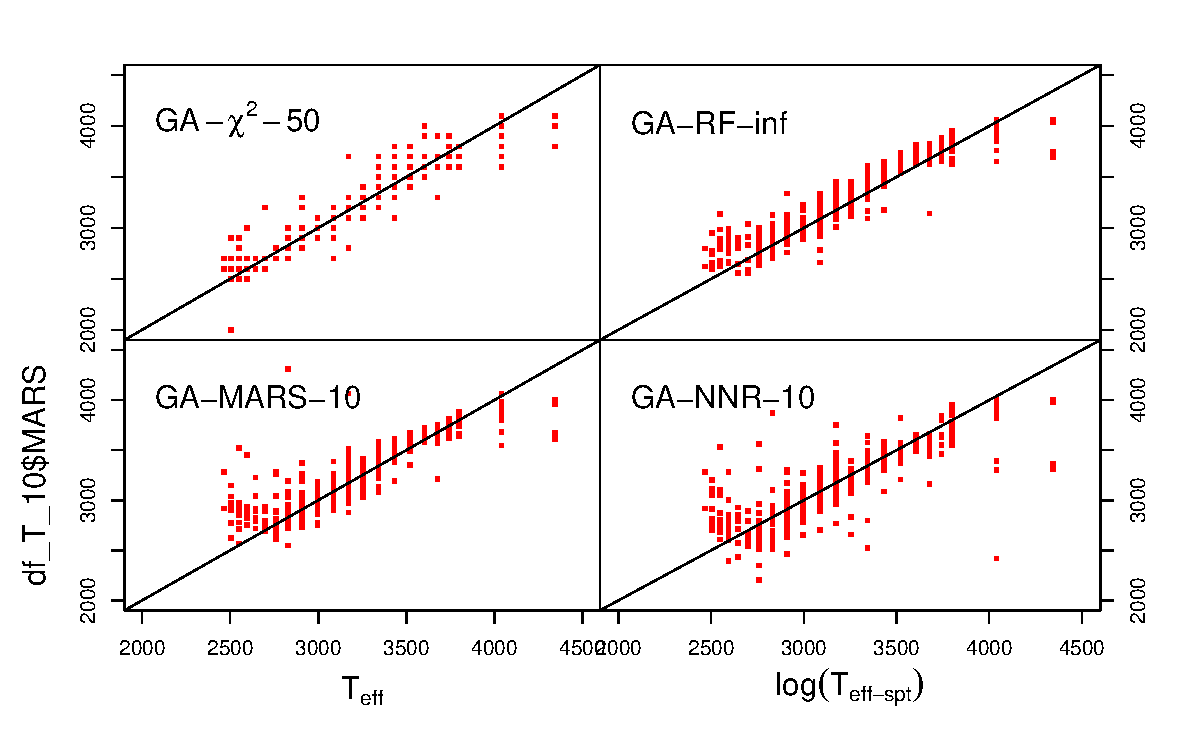
\includegraphics[width=\textwidth]{figs/ipac-teff}
\caption{Comparison
 between the effective temperatures derived from the tabulated
 spectral types in \protect\cite{cesetti} ($x$ axis) and those
 inferred by the various regression modules ($y$ axis): $\chi^2$
 module (top left, SNR=50), Random Forest Regression module (top
 right, SNR=$\infty$), GA-MARS module (bottom left, SNR=10), and the
 Neural Network module (bottom right, SNR=10).  Blue squares denote
 Main Sequence dwarfs and red triangles denote giant stars (luminosity
 class III) according to \protect\cite{cesetti}} \label{fig:ipac_teff}
\end {figure*}

Having shown that the feature selection with GAs degrades the
performance of regression models, one can wonder whether a different
feature selection procedure would produce better results. In
particular, we investigate the possibility that the features proposed
by \cite{cesetti} result in a performance equal to or even better than
the one achieved with $\chi^2$.

We train the same types of regression models to the features selected
in \cite{cesetti}, again learning from BT-Settl spectra of various
SNRs and predicting over the Dwarf Archives set. A summary of the results can be
found in Table \ref{tab:ipac-teff-rmse-cesetti}, where we use CS- to
indicate that the model was trained using the features
by \cite{cesetti}. 

For SNR=10, the best GA models (GA-KPLS in RMDSE or GA-RF in RMSE)
outperform the best CS model (GA-GBM). For SNR=50 the situation
depends on the figure-of-merit used to compare the regression models:
in RMSE the best model is CS-GBM while in RMDSE GA-GBM outperforms all
CS-models. Finally, for the unrealistic case of noiseless spectra,
Table \ref{tab:ipac-teff-rmse-cesetti} shows an overwhelming
degradation of the prediction accuracy from CS- features. But even in
the only case where the CS features outperform those selected by the
GA, the performance is below the one achieved by the minimum-$\chi^2$
approach. It is important to remark here that the features selected
in \cite{cesetti} were fit for the IRTF wavelength range and
resolution, and not all of them can be extracted from Dwarf Archives 
spectra. Hence, unlike in the case of the IRTF spectra, the comparison
of GA- and CS-based performances with Dwarf Archives spectra is not fair and the
results are only included for the sake of completeness.

The relationship between the GA predicted effective temperature and
the one measured by \cite{RA2012} (blue for the predictions by the
GA-MARS SNR=10 model and black for GA-RF SNR=$\infty$ model), and
by \cite{esm1} and \cite{esm2} (orange and green for
the same models as before) can be found in
Figure~\ref{fig:ipac_lt_lt}.

\begin{figure}
 \begin{center} 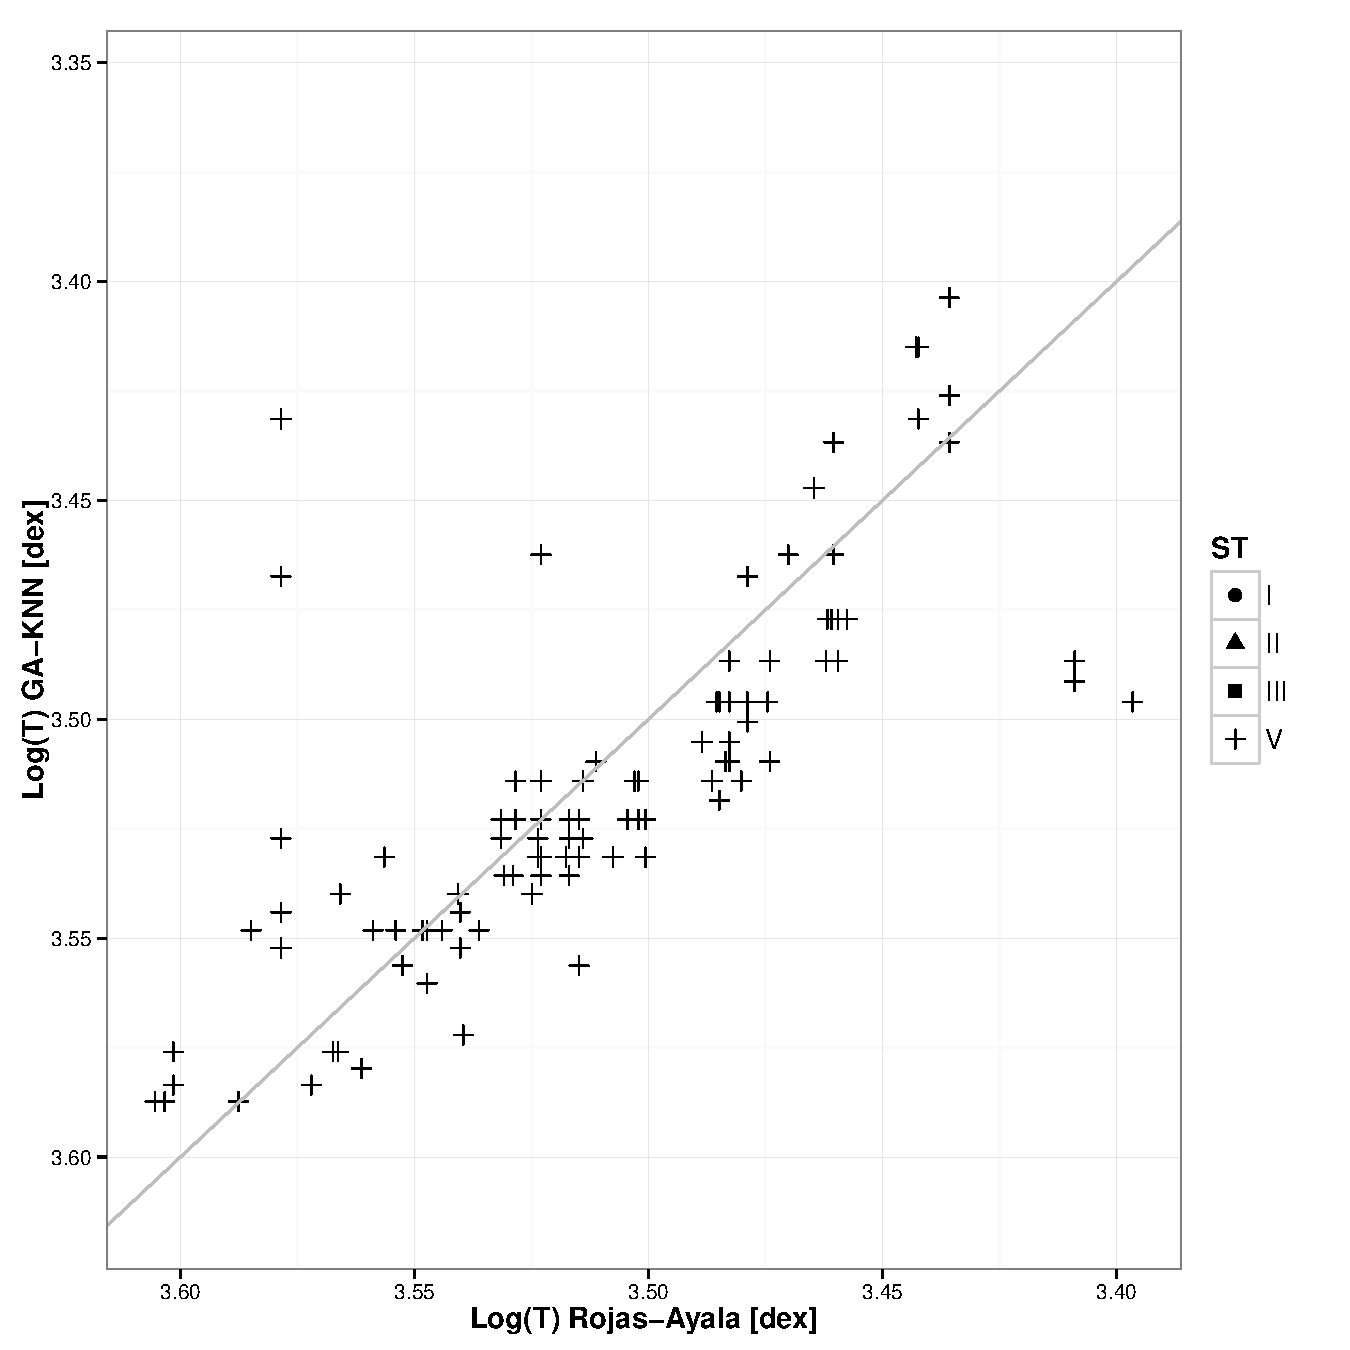
\includegraphics[width=8cm]{figs/ipac_LG_Trojas_Tknn_10}

\caption{Relationship  between $\log(T_{\rm eff})$ from \protect\cite{RA2012}
in the $x$ axis and $\log(T_{\rm eff})$ as predicted by the GA-RF
 model with SNR=$\infty$ (black symbols, squares for dwarfs and a
 triangle for the only giant in the sample) and the GA-MARS trained
 with SNR=10 data (blue symbols). Green and orange symbols correspond
 to sources in common with \protect\cite{esm1}
 and \protect\cite{esm2} and the predictions by the
 GA-RF (SNR=$\infty$) and GA-MARS (SNR=10) models
 respectively.} \label{fig:ipac_lt_lt} \end{center}
\end{figure}



\subsubsection{Surface gravity models}

As in the IRTF exercise, we attempt to select features for surface
gravity estimation from BT-Settl spectra using GAs despite the much
lower spectral resolution and smaller wavelength coverage of the Dwarf Archives
spectra. Since there is no substantive compilation of surface
gravities that we could cross match with the IPAC list of M stars in
the Dwarf Archive, we are left with the same plausibility arguments
used in the IRTF study which are based on the $\log(T_{\rm
eff})$--$\log(g)$ diagram.

We again use the effective temperatures as input of the regression
models. Table~\ref{tab:ipac-logg-rmse} shows the cross-validation RMSE
and RMDSE for the same set of regression models used throughout this
article. It shows that the GA-RF model outperforms all other in all
SNR regimes, giving a consistent RMDSE of 1.0 dex. Obviously, this is
barely enough for classification in luminosity classes. Furthermore,
and as has been the case in the evaluation of all previous regression
modules, the cross-validation errors are poor estimates of the true
performances on real observed spectra. Figure \ref{fig:teffvsloggIPAC}
shows the $\log(T_{\rm eff})$--$\log(g)$ diagram for the best two
performing $\log(g)$ regression models (GA-NNR and GA-SVR, both
trained with SNR=10 BT-Settl spectra) and the two reference modules
based on the minimization of the $\chi^2$ (SNR=50) and the PPR-ICA
(SNR=10). Three of the four panels (all except the $\chi^2$
predictions) show a strong spurious correlation in the gravities of
the M dwarfs in the sense that the coolest dwarfs have unreasonable
values of $\log(g)$ around 2 dex. The PPR-ICA model shows this trend
too, but with a much shallower slope ($\log(g)\approx 4$ at
$\log(T_{\rm eff})\approx 3.4$). Only the GA-NNR module (and to a
lesser extent the $\chi^2$ module) places giant stars (red triangles)
in the locus expected judging by the values in Table 3
of \cite{cesetti} (black filled symbols) and the predictions for the
IRTF data set (green filled symbols). The various symbols (squares,
triangles, circles) reflect the luminosity classes found in either
Table 3 of \cite{cesetti} (for the IRTF values) or the DwarfArchives
table. 


\begin{figure*}
 \begin{center}
 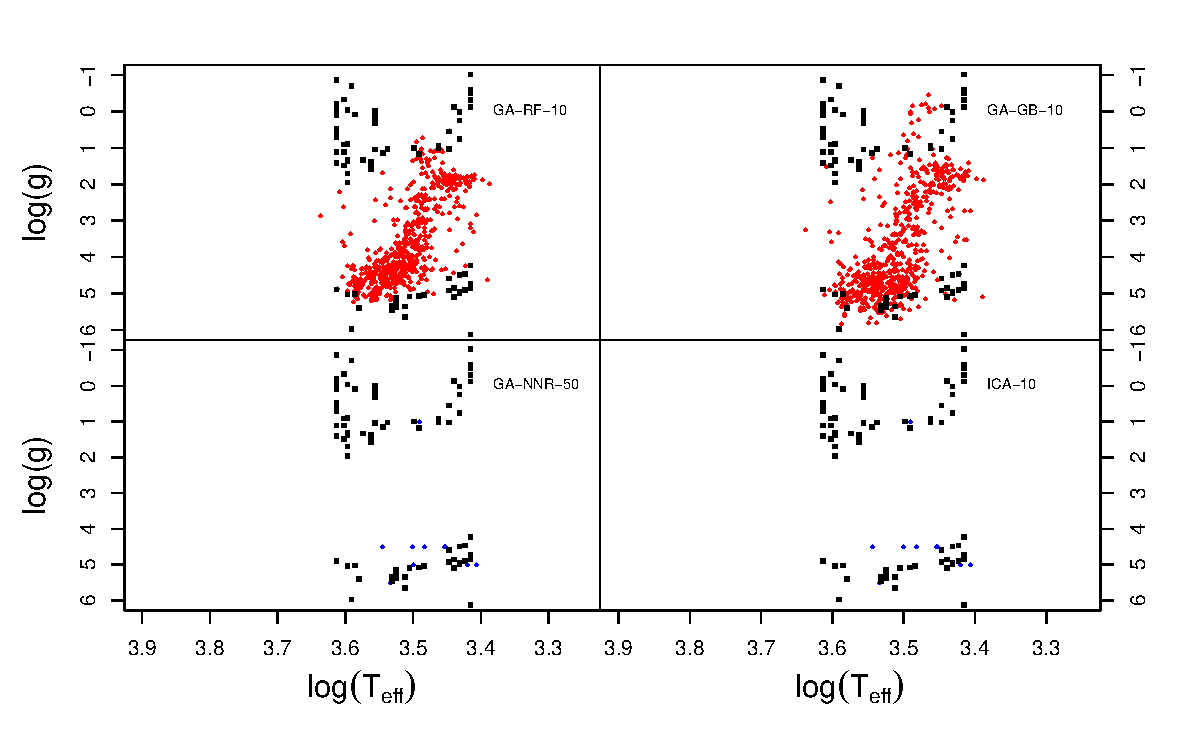
\includegraphics[width=\textwidth]{figs/ipac-teff-logg}

\caption{$\log(T_{\rm eff})$-$\log(g)$ planes obtained using the $\chi^2$ (SNR=50)
$\log(T_{\rm eff})$ preditions and the $\log(g)$ values from the
GA-NNR (SNR=10, top left), GA-SVR (SNR=10, top right), $\chi^2$
(SNR=50, bottom left), and PPR-ICA (SNR=10, bottom right) regression
models. Black symbols correspond to objects with physical parameters
in Table 3 of \protect\cite{cesetti}; green symbols correspond to the
predictions shown in Section \ref{sect:irtf-teff} for the IRTF
spectra; blue squares correspond to predictions for dwarf stars
according to the DwarfArchives.org luminosity classes; red triangles
correspond to giant stars according to DwarfArchives.org; orange
symbols correspond to values derived from high-resolution infrared
spectra by \protect\cite{esm1} and \protect\cite{esm2};
and finally, empty grey circles correspond to sources with no
luminosity class in DwarfArchives.org.}

\label{fig:teffvsloggIPAC}
 \end{center}
\end{figure*}

\subsubsection{Metallicity models} 

Finally, the same analysis is performed for metallicities, again using
the previously inferred temperature as a fixed input feature.
Table~\ref{tab:ipac-met-rmse} shows a summary of the cross-validation
performance of the different models.

In general, models trained with SNR=$\infty$ show much poorer
performace except for the GA-RF and GA-GBM cases. The best $\chi^2$
model produces errors almost a factor two larger than the
$GA-RF-\infty$ model (although it has to be borne in mind that, while
our regression models are capable of predicting metallicities that are
intermediate in the grid, the minimum $\chi^2$ can only yield values
in the grid, which has a step size of 0.5 dex). Models trained with
SNR=10 and 50, on the contrary, show a more consistent behaviour for
the entire set of regressors, with poorer performances than the
apparently optimal $GA-RF-\infty$, but also smaller differences
between models.

In order to select the best model, we again compare our model
predictions with the reference catalogs used in
Sect. \ref{sect:irtf-met}. We select the Random Forest trained with
noiseless synthetic spectra as the best model, which renders the
minimum RMSE (0.3 dex). Figure \ref{fig:ipac_mt} shows the comparison
of our estimates with the reference catalogs, using the same symbols
and colours as in Fig. \ref{MIRTF_ICA_10}.

Our value of the RMSE contrasts with the differences between estimates
for the same star in the literature. We obtain a mean difference of
0.1 dex a factor 3 smaller than our RMSE. 

\begin{figure}
 \begin{center} 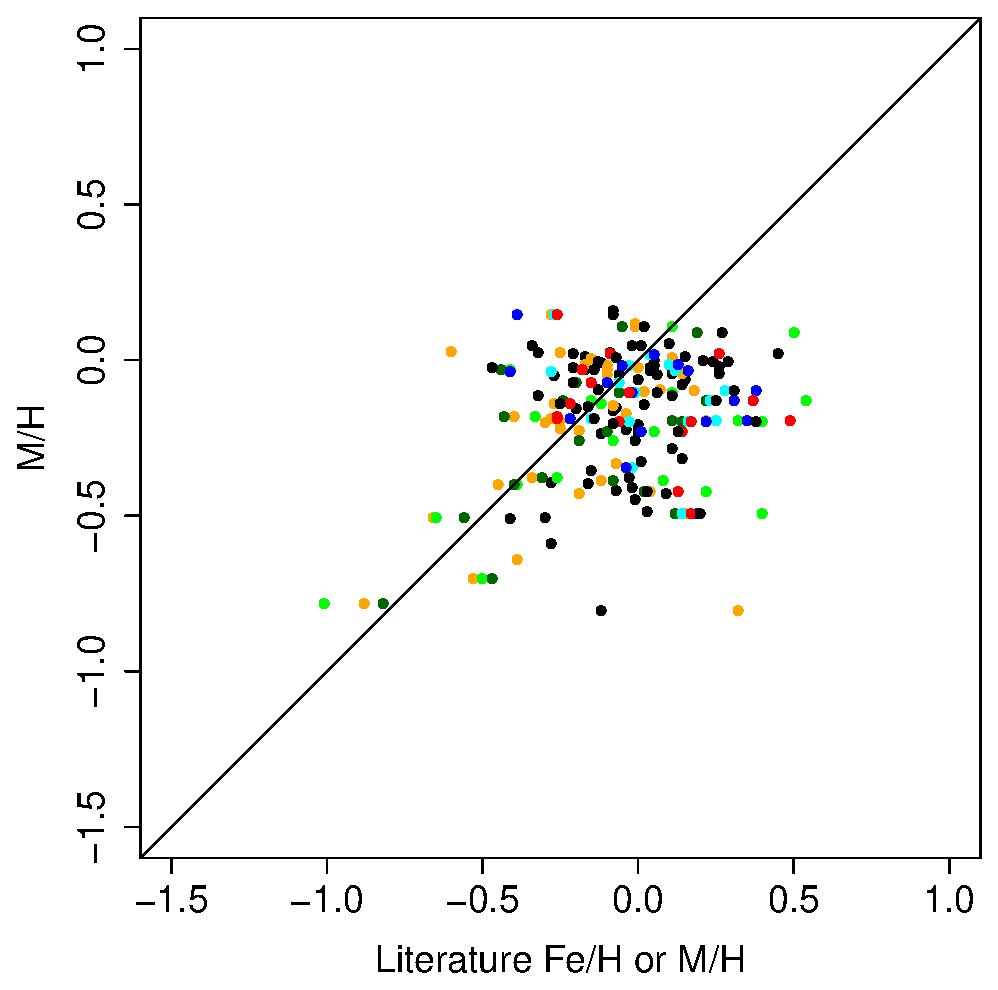
\includegraphics[width=8cm]{figs/ipac-figs/M-RFInf}

\caption{Relationship
 between the $RF-\infty$ predictions for metallicity and values from
 the literature for stars in the Dwarf Archives.  Black symbols
 represent values from \protect\cite{cesetti} ; orange symbols, values
 from \protect\cite{NevesIII}; green symbols, values that the Vizier
 catalog entry for Table 8 of \protect\cite{NevesIII} links
 to \protect\cite{Jao}, although we find no evidence
 that \protect\cite{Jao} contains estimates of metallicities; cyan and
 blue symbols, the values of [M/H] and [Fe/H] respectively
 in \protect\cite{RA2012}; red symbols, values
 from \protect\cite{Mann2015}; yellow symbols, values
 from \protect\cite{Newton2014}; and, finally, black symbols, values
 from \protect\cite{Gaidos2015}.}  \label{fig:ipac_mt} \end{center}
\end{figure}


It is interesting to note that our predictions extend to metallicities
as low as [M/H]=-2.1. Figure \ref{fig:ipac-hist-mets} shows a histogram of
the metallicities predicted by the GA-RF-$\infty$ model for the Dwarf Archives 
set of spectra. We find predictions below -1.5 for eleven sources, 6
of which have been previously identified as subdwarfs of different
categories (see Table \ref{tab:known-sds}).

\begin{figure}
	\begin{center}
		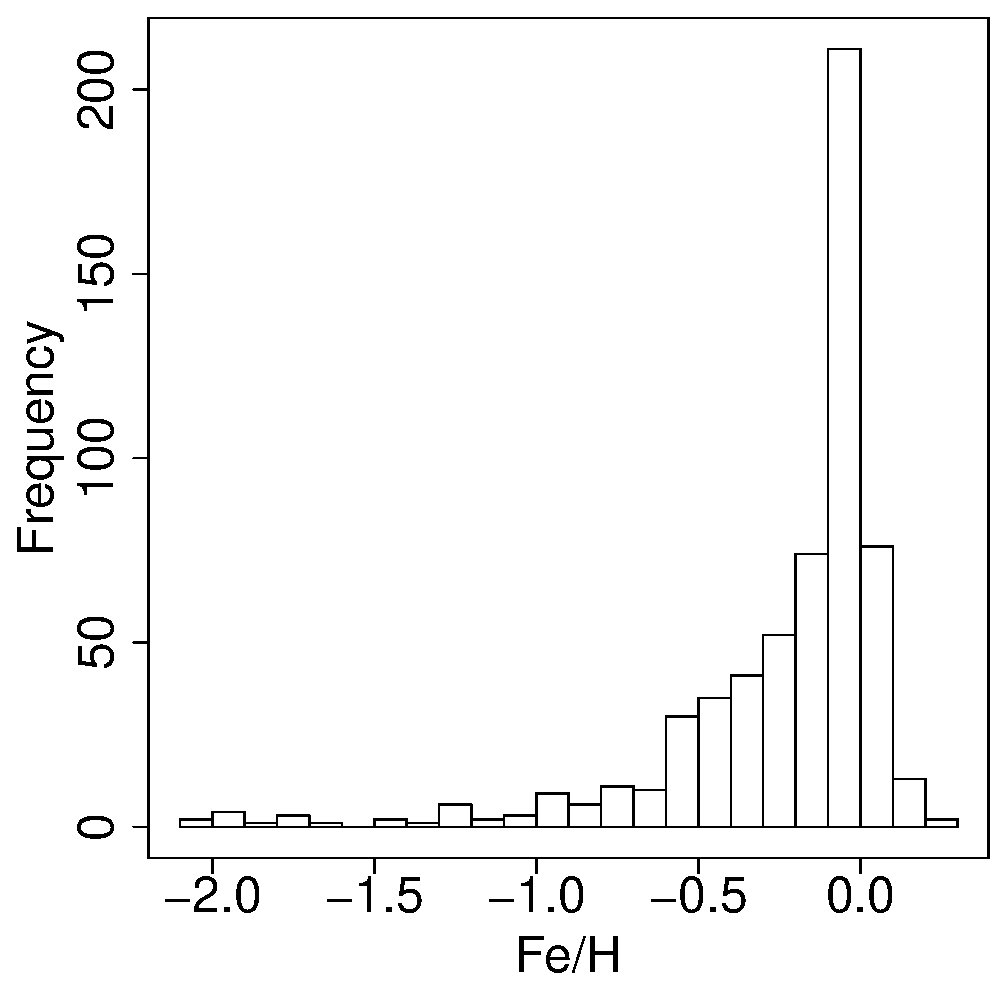
\includegraphics[width=8cm]{figs/ipac-figs/ipac-M-hist}

	\end{center}
        
        \caption{\label{fig:ipac-hist-mets}
Predictions of the GA-RF-$\infty$ regression model
        for the metallicity of Dwarf Archives stars.}

\end{figure}


\begin{table}\centering
	\begin{tabular}{@{}llll@{}}
		\hline
		Identifier & classification & Reference & GA-RF-$\infty$\\
		\hline
		LHS 3768 & usdM3 & \cite{1995AJ....109..797K}  & -2.1 \\
		LHS 2352 & esd   & \cite{1995AJ....109..797K}  & -2.0 \\
		LHS 1691 & usdM2 & \cite{0004-637X-669-2-1235} & -1.95\\
		LHS 2023 & esdM6 & \cite{0004-637X-672-2-1153} & -1.95\\
		LHS 515  & esdM5 & \cite{1538-3873-117-833-676}& -1.8\\
		LP471-17 & sdM   & \cite{1995AJ....109..797K}  & -1.7\\
		\hline
	\end{tabular}
        
	\caption{Previously known subdwarfs in the Dwarf Archives collection of
	spectra and the corresponding GA-RF-$\infty$ predictions.}

\label{tab:known-sds} 
\end{table}

The remaining 5 stars with metallicities below -1.5 are 2MASS
J17275631-3240430 (-2.0 dex); LHS 1625 (-1.97 dex); 2MASS
J19215188+2802275 (-1.9 dex); 2MASS J19004675+2806462 (-1.7 dex),
classified as K7III by \cite{1994ApJS...94..749K}); and 2MASS
J14465233-5320580 (-1.7 dex).

